\documentclass[UTF8,a4paper,zihao=-4]{ctexart}
\usepackage{amsmath,amssymb}
\usepackage{geometry}
\usepackage{hyperref}
\usepackage{enumitem}
\usepackage{xcolor}
\usepackage{graphicx}
\setmainfont{Times New Roman}
\geometry{left=2.8cm,right=2.8cm,top=2.8cm,bottom=2.8cm}
\hypersetup{unicode=true,colorlinks=true,linkcolor=blue,urlcolor=blue}
\setlist[enumerate]{itemsep=0.2em,topsep=0.4em}
\setlength{\parindent}{2em}
\setlength{\parskip}{0.35em}
\setcounter{secnumdepth}{0}
\title{具有线性动力学的最优控制终端问题的数值解}
\author{}
\date{}
\begin{document}
\maketitle
\tableofcontents
\newpage

\section{摘要}

本文研究具有线性动力学的最优控制终端问题的数值解。研究对象为常系数线性控制系统

\[
\dot{x}(t)=Ax(t)+Bu(t),\quad x(0)=x_0,\quad u(t)\in U,\quad t\in[0,T],
\]

其中 $A$ 与 $B$ 为给定常数矩阵，$U$ 为非空紧凸控制集。论文围绕两个终端型问题展开：一是二次终端误差最小化问题，二是带仿射终端目标集约束的线性终端泛函最小化问题。首先建立线性系统解公式、允许控制集、可达集和支撑函数等基础概念；其次在统一的最小化框架下引入最大化形式伴随变量 $\psi=-p$，将最大值条件写成支撑函数上的线性最大化问题；然后利用线性伴随方程的结构，用终端伴随向量 $q=\psi(T)$ 或乘子 $\lambda$ 参数化整条伴随轨线、控制函数和状态轨线；最后把原无限维控制函数优化问题转化为有限维残差最小二乘问题，并给出离散递推、有限差分 Jacobian、Armijo 线搜索、高斯--牛顿迭代和光滑化处理等可实现的数值算法。数值实验部分通过一维系统、二维终端跟踪、仿射终端约束和非光滑控制集光滑化对比等算例，验证算法在终端误差、终端约束残差、目标函数下降和控制曲线稳定性方面的效果。

\section{关键词}

最优控制；线性动力学；终端问题；数值解；庞特里亚金最大值原理；伴随方程；支撑函数；有限维参数化；高斯--牛顿法

\section{第1章 绪论}

\subsection{1.1 研究背景与意义}

最优控制理论研究如何在给定动力系统、约束条件和性能指标下选择控制函数，使系统运动达到某种最优效果\cite[第13--27页]{pontryagin1969}\cite[第76--91页]{lee1972}\cite[第8--15页]{blagodatskikh2001}。在线性动力学系统中，状态方程具有较清晰的解析结构，矩阵指数、可达集、支撑函数和伴随方程都可以得到相对明确的表达，因此线性系统既是最优控制理论的重要基础，也是构造数值算法的重要对象。

终端型最优控制问题关注系统在终端时刻的状态表现。例如，使终端状态尽可能接近目标点，或者要求终端状态落入指定目标集，同时使某个终端性能指标最优。这类问题广泛出现在轨迹规划、导航控制、经济过程控制、工程系统调节和资源优化等问题中。

本文的研究意义在于：利用线性动力学和伴随方程的结构特点，将原本关于控制函数的无限维优化问题转化为关于有限维参数的优化问题，并进一步构造可计算的数值求解流程\cite[第180--190页]{kiselev2007}\cite[第5--7页]{avvakumov1995}。这样既能体现庞特里亚金最大值原理的理论作用，也能为终端型最优控制问题提供实际可实现的计算方法。

\subsection{1.2 国内外研究现状}

与本文相关的研究可以从最优性条件、线性系统几何结构、数值求解方法和本文定位四个方面理解。

第一，庞特里亚金最大值原理为最优控制问题提供了伴随方程、Hamilton 函数最大化条件和横截条件等必要条件\cite[第23--27页]{pontryagin1969}\cite[第336--371页]{lee1972}\cite[第119--158页]{pontryagin1985}。后续教材和专著进一步系统化了变分法、正常与异常极值、终端约束和法锥条件等内容\cite{bryson1975,kirk1970,vinter2000,liberzon2012}。这些理论说明，终端型问题通常不能只看状态方程本身，还必须同时处理伴随变量和终端横截条件。

第二，在线性控制系统中，状态对控制的依赖是线性的，可达集在紧凸控制集作用下具有凸几何结构\cite[第15--59页]{kiselev2007}\cite[第76--91页]{lee1972}。支撑函数方法可以把控制集上的线性最大化写成 $c_U(\eta)=\max_{u\in U}\langle\eta,u\rangle$，从而把最大值条件与可达集的支撑超平面联系起来\cite[第29--37页]{blagodatskikh2001}\cite[第3--4页]{avvakumov1995}。这一路线特别适合分析终端误差最小化和仿射终端约束下的线性泛函优化。

第三，数值最优控制方法大体可分为直接法和间接法。直接法把控制或状态轨线离散化后转化为非线性规划问题，具有实现稳健、便于处理复杂约束的特点\cite{betts2010,rao2009}；间接法先利用最大值原理得到边值问题或低维参数方程，通常维数较低，但对初值、非光滑性和切换结构更敏感\cite[第180--190页]{kiselev2007}\cite[第3--10页]{avvakumov1995}。有限差分 Jacobian、线搜索、高斯--牛顿和阻尼迭代属于常用的数值优化工具\cite{nocedal2006,kelley1999}，可用于求解由间接法得到的有限维残差方程。

本文采用间接法与有限维参数优化相结合的路线。与直接把每个时间节点控制值作为优化变量的做法不同，本文先由最大值原理确定控制结构，再利用线性伴随方程把未知量压缩为终端伴随向量 $q$ 或乘子 $\lambda$。这样既保留了最大值原理的理论解释，又能形成可复现的有限维最小二乘数值算法。为避免只从单一算法角度解释数值结果，实验部分还加入一个直接离散优化对比算例，用同一 Euler 离散格式和同一盒约束检验终端目标的可达性及间接参数化方法的适用边界。

\subsection{1.3 本文研究内容}

本文只固定研究以下两个主问题。

第一个主问题为二次终端误差最小化问题：

\[
\dot{x}(t)=Ax(t)+Bu(t),\quad x(0)=x_0,\quad u(t)\in U
\]

\[
J_1(u)=\frac{1}{2}\|x(T;u)-x_T\|^2\to\min
\]

其中 $x_T\in\mathbb{R}^n$ 为给定终端目标点。该问题的目标是选择允许控制 $u(\cdot)$，使终端状态 $x(T;u)$ 尽量接近 $x_T$。

第二个主问题为带终端目标集约束的线性终端泛函最小化问题：

\[
\dot{x}(t)=Ax(t)+Bu(t),\quad x(0)=x_0,\quad u(t)\in U
\]

\[
x(T;u)\in M
\]

\[
J_2(u)=a^\top x(T;u)\to\min
\]

其中 $a\in\mathbb{R}^n$ 为给定向量，$M\subset\mathbb{R}^n$ 为终端目标集。该问题要求终端状态满足集合约束，并在可行终端状态中优化线性终端指标。

本文主要完成以下工作：

\begin{enumerate}
\item 建立具有线性动力学的终端型最优控制问题的数学模型。
\item 给出允许控制集、可达集、支撑函数和终端性能指标的基本定义。
\item 统一最小化问题的符号约定，引入最大化形式的伴随变量。
\item 推导两个主问题对应的伴随方程、最大值条件和终端条件。
\item 解释有限维参数化思想，将未知控制函数转化为有限维伴随终端参数。
\item 构造面向两个主问题的有限维残差方程、离散递推格式和可实现迭代算法。
\item 通过数值算例分析算法的终端误差、终端约束残差、目标函数下降、控制曲线和参数敏感性。
\end{enumerate}

\subsection{1.4 本文主要特点}

本文的主要特点体现在以下三个方面。

\begin{enumerate}
\item 研究范围固定在两个终端型问题上，避免把论文写成一般最优控制理论综述。
\item 数值求解以伴随终端参数为优化变量，不把每个时间节点的控制值都作为独立优化变量，从而保持有限维参数化方法的主题。
\item 算法部分给出离散状态递推、残差函数、Jacobian 近似、线搜索、停止准则和实验指标，使数值解部分具备可复现性。
\end{enumerate}

\subsection{1.5 本文结构安排}

第1章介绍研究背景、研究现状、研究内容和论文结构。

第2章建立线性控制系统、矩阵指数、可达集、支撑函数和两个主问题的数学基础，并给出全文使用的基本假设。

第3章在统一最小化框架下推导终端型线性最优控制问题的最优性条件，包括伴随方程、最大值条件、终端条件和有限维参数化思想。

第4章构造基于最大值原理的数值求解方法，给出时间离散、控制生成公式、有限维残差、有限差分 Jacobian、Armijo 线搜索、高斯--牛顿型迭代和非光滑控制集的光滑化处理。

第5章通过多个线性系统算例验证算法效果，分析终端误差、目标函数变化、控制曲线、状态轨线和算法收敛性。

第6章总结全文工作，并讨论进一步研究方向。

\section{第2章 线性控制系统与终端型最优控制问题的数学基础}

\subsection{2.1 线性控制系统}

考虑有限维常系数线性控制系统\cite[第15--31页]{kiselev2007}\cite[第76--91页]{lee1972}：

\[
\dot{x}(t)=Ax(t)+Bu(t),\quad t\in[0,T]
\]

\[
x(0)=x_0
\]

其中 $x(t)\in\mathbb{R}^n$，$u(t)\in\mathbb{R}^m$，$A\in\mathbb{R}^{n\times n}$，$B\in\mathbb{R}^{n\times m}$ 为给定常数矩阵。本文后续推导均以该常系数线性系统为基础。

\subsection{2.2 矩阵指数与系统解公式}

对于常系数线性系统：

\[
\dot{x}(t)=Ax(t)+Bu(t),\quad x(0)=x_0
\]

齐次系统 $\dot{x}(t)=Ax(t)$ 的解由矩阵指数 $e^{At}$ 给出\cite[第15--31页]{kiselev2007}\cite[第76--91页]{lee1972}。由常数变易公式，受控系统的解为：

\[
x(t)=e^{At}x_0+\int_0^t e^{A(t-s)}Bu(s)\,ds
\]

因此终端状态满足：

\[
x(T)=e^{AT}x_0+\int_0^T e^{A(T-s)}Bu(s)\,ds
\]

该公式说明，在常系数线性系统中，终端状态由初始状态和控制函数共同决定，并且控制函数以线性方式影响终端状态。这是后续讨论可达集、支撑函数和有限维参数化的基础。
\subsection{2.3 允许控制集与可达集}

设控制约束集为：

\[
U\subset\mathbb{R}^m
\]

允许控制集合定义为满足控制约束的本质有界可测函数集合，记为：

\[
\mathcal{U}=L_\infty([0,T];U)
\]

等价地，对任意允许控制，有：

\[
u(\cdot)\in L_\infty([0,T];U)
\]

终端时刻 $T$ 的可达集定义为：

\[
X(T)=\{x(T;u):u(\cdot)\in\mathcal{U}\}
\]

由线性系统解公式可知：

\[
X(T)=e^{AT}x_0+
\left\{
\int_0^T e^{A(T-s)}Bu(s)\,ds:
u(\cdot)\in\mathcal{U}
\right\}
\]






当 $U$ 为非空紧凸集时，控制对终端状态的作用是线性积分映射，因此可达集具有凸性；在本文采用的有限维常系数系统和有界控制设定下，可达集具有适合投影和支撑超平面分析的闭凸结构\cite[第76--91页]{lee1972}\cite[第32--40页]{kiselev2007}。终端型最优控制问题可以理解为在可达集 $X(T)$ 上优化某个终端函数，或在可达集与终端目标集的交集中寻找最优终端点。

\subsection{2.4 支撑函数}

对非空紧凸集 $U\subset\mathbb{R}^m$，定义其支撑函数\cite[第29--37页]{blagodatskikh2001}\cite[第3--4页]{avvakumov1995}：

\[
c_U(\eta)=\max_{u\in U}\langle \eta,u\rangle,\quad \eta\in\mathbb{R}^m
\]

其中 $\langle\cdot,\cdot\rangle$ 表示欧氏内积。由于 $U$ 非空紧，最大值可以取到。

支撑函数用于描述控制约束集上的线性最大化问题\cite[第3--4页]{avvakumov1995}。在最大值原理中，最优控制通常满足：

\[
u^*(t)\in\arg\max_{u\in U}\langle B^\top\psi(t),u\rangle
\]

因此有：

\[
\langle B^\top\psi(t),u^*(t)\rangle=c_U(B^\top\psi(t))
\]

若 $U$ 为光滑严格凸集，则 $c_U$ 可微，最优控制可以写为：

\[
u^*(t)=\nabla c_U(B^\top\psi(t))
\]

若 $U$ 为区间、盒约束或多面体，则 $c_U$ 一般不可微，最优控制可能出现开关结构。
此时可采用次梯度、多值最大化选择或光滑化近似。


\subsection{2.5 本文研究的两个主问题}

本文只研究两个终端型问题。

问题一为二次终端误差最小化问题：

\[
\begin{cases}
\dot{x}(t)=Ax(t)+Bu(t),\\
x(0)=x_0,\\
u(t)\in U,
\end{cases}
\]

\[
J_1(u)=\frac{1}{2}\|x(T;u)-x_T\|^2\to\min
\]

该问题可以看作在可达集 $X(T)$ 中寻找距离目标点 $x_T$ 最近的终端状态。如果 $x_T\in X(T)$，则最优终端误差可以为零；如果 $x_T\notin X(T)$，则最优解对应于可达集上离 $x_T$ 最近的点。

问题二为带终端目标集约束的线性终端泛函最小化问题：

\[
\begin{cases}
\dot{x}(t)=Ax(t)+Bu(t),\\
x(0)=x_0,\\
u(t)\in U,\\
x(T)\in M,
\end{cases}
\]

\[
J_2(u)=a^\top x(T;u)\to\min
\]

其中 $M$ 为给定终端目标集。本文重点考虑 $M$ 为仿射集合的情形：

\[
M=\{x\in\mathbb{R}^n:Cx=d\}
\]

此时终端约束可以用有限个线性方程描述，便于写出横截条件和参数化形式。

\subsection{2.6 本章小结}

本章建立了线性控制系统、矩阵指数、允许控制集、可达集和支撑函数等基本概念，并明确了本文研究的两个主问题。后续章节将在这些定义的基础上，推导最优性条件并构造数值求解方法。

\section{第3章 终端型线性最优控制问题的最优性条件}

\subsection{3.1 最小化问题的统一表述}

本文所有原始优化问题统一写成最小化形式：

\[
J(u)\to\min
\]

对一般终端型问题，可写为：

\[
\dot{x}(t)=Ax(t)+Bu(t),\quad x(0)=x_0,\quad u(t)\in U
\]

\[
J(u)=\Phi(x(T))\to\min
\]

若存在终端约束，则补充：

\[
x(T)\in M
\]

为了使用支撑函数 $c_U(\eta)=\max_{u\in U}\langle\eta,u\rangle$，本文引入最大化形式的伴随变量。设最小化问题中常规伴随变量为 $p(t)$，定义：

\[
\psi(t)=-p(t)
\]

这样可以将控制条件统一写成控制集上的最大化问题。

\subsection{3.2 Hamilton 函数与伴随方程}

采用最大化形式伴随变量 $\psi(t)$，定义 Hamilton 函数为：

\[
H(x,u,\psi,t)=\langle \psi,Ax+Bu\rangle
\]

由于系统关于状态变量线性，伴随方程为：

\[
\dot{\psi}(t)=-A^\top\psi(t)
\]

给定终端伴随向量：

\[
q=\psi(T)
\]

则伴随方程的解为：

\[
\psi(t,q)=e^{A^\top(T-t)}q
\]

因此，在线性动力学下，整条伴随轨线由有限维向量 $q=\psi(T)$ 决定。

\subsection{3.3 最大值条件与支撑函数表示}

庞特里亚金最大值原理给出控制条件\cite[第23--27页]{pontryagin1969}\cite[第336--371页]{lee1972}\cite[第8--15页]{blagodatskikh2001}：

\[
H(x^*(t),u^*(t),\psi(t),t)
=
\max_{u\in U}H(x^*(t),u,\psi(t),t)
\]

由于 $u$ 在 Hamilton 函数中线性出现，该条件等价于：

\[
u^*(t)\in\arg\max_{u\in U}
\langle B^\top\psi(t),u\rangle
\]

利用支撑函数，可写为：

\[
\langle B^\top\psi(t),u^*(t)\rangle
=
c_U(B^\top\psi(t))
\]

若 $c_U$ 可微，则最优控制具有显式表达：

\[
u^*(t)=\nabla c_U(B^\top\psi(t))
\]

这说明只要确定伴随变量 $\psi(t)$，便可以由最大值条件确定控制函数 $u^*(t)$。

\subsection{3.4 二次终端误差问题的终端条件}

问题一的性能指标为：

\[
J_1(u)=\frac{1}{2}\|x(T;u)-x_T\|^2
\]

记：

\[
\Phi_1(x)=\frac{1}{2}\|x-x_T\|^2
\]

则：

\[
\nabla\Phi_1(x)=x-x_T
\]

对最小化伴随变量 $p(t)$，终端条件为：

\[
p(T)=x^*(T)-x_T
\]

由于本文使用：

\[
\psi(t)=-p(t)
\]

因此最大化形式伴随变量的终端条件为：

\[
\psi(T)=x_T-x^*(T)
\]

令 $q=\psi(T)$，则问题一可以理解为寻找 $q$，使由 $q$ 生成的控制和状态满足：

\[
q=x_T-x(T,q)
\]

该关系为后续构造参数优化方法提供依据。

\subsection{3.5 终端目标集问题的横截条件}

问题二为：

\[
J_2(u)=a^\top x(T;u)\to\min,\quad x(T)\in M
\]

若 $M$ 为一般闭凸集，则最小化伴随变量 $p(t)$ 满足\cite[第121--127页]{pontryagin1969}\cite[第336--371页]{lee1972}：

\[
p(T)\in a+N_M(x^*(T))
\]

其中 $N_M(x^*(T))$ 是集合 $M$ 在 $x^*(T)$ 处的法锥。由于 $\psi(t)=-p(t)$，最大化形式伴随变量满足：

\[
\psi(T)\in -a-N_M(x^*(T))
\]

当 $M$ 为仿射集合：

\[
M=\{x\in\mathbb{R}^n:Cx=d\}
\]

其法空间为 $\operatorname{Range}(C^\top)$。因此存在乘子 $\lambda$，使：

\[
p(T)=a+C^\top\lambda
\]

于是：

\[
\psi(T)=-a-C^\top\lambda
\]

若用矩阵 $H$ 表示终端约束法空间的一组基，也可以写成：

\[
\psi(T)=-a-H\lambda
\]

这说明问题二中的未知伴随终端向量可以由有限维参数 $\lambda$ 表示。

\subsection{3.6 有限维参数化思想}

原始最优控制问题的未知量是控制函数：

\[
u(\cdot):[0,T]\to U
\]

这个未知量属于函数空间，因此原问题本质上是无限维优化问题。

在线性动力学下，伴随方程为\cite[第23--27页]{pontryagin1969}\cite[第5--7页]{avvakumov1995}：

\[
\dot{\psi}(t)=-A^\top\psi(t)
\]

整条伴随轨线由终端向量：

\[
q=\psi(T)\in\mathbb{R}^n
\]

唯一决定。具体有：

\[
\psi(t,q)=e^{A^\top(T-t)}q
\]

再由最大值条件：

\[
u(t,q)\in\arg\max_{u\in U}
\langle B^\top\psi(t,q),u\rangle
\]

即可得到由 $q$ 生成的控制函数。若 $c_U$ 可微，则：

\[
u(t,q)=\nabla c_U(B^\top\psi(t,q))
\]

然后将 $u(t,q)$ 代入状态方程，得到：

\[
\dot{x}(t,q)=Ax(t,q)+Bu(t,q),\quad x(0,q)=x_0
\]

从而得到终端状态：

\[
x(T,q)
\]

因此有如下对应关系：

\begin{verbatim}
有限维向量 q
  -> 伴随轨线 psi(t,q)
  -> 控制函数 u(t,q)
  -> 状态轨线 x(t,q)
  -> 终端状态 x(T,q)
\end{verbatim}

这就是有限维参数化的含义：原来需要在所有控制函数 $u(\cdot)$ 中寻找最优控制，现在转化为在有限维向量 $q$ 或 $\lambda$ 中寻找最优参数\cite[第180--190页]{kiselev2007}\cite[第5--7页]{avvakumov1995}。实际数值计算仍然需要对时间区间进行离散化，但优化变量不再是每个时间节点上的控制值，而是低维的伴随终端参数。

对于问题一，主要参数为：

\[
q=\psi(T)
\]

对于问题二，在仿射终端约束下可以取：

\[
q(\lambda)=-a-C^\top\lambda
\]

或：

\[
q(\lambda)=-a-H\lambda
\]

于是问题二转化为关于 $\lambda$ 的有限维优化问题。

\subsection{3.7 本章小结}

本章统一了全文的符号方向：原始问题均写成最小化形式，并通过 $\psi=-p$ 引入最大化形式的伴随变量，使控制条件能够用支撑函数表示。随后分别给出了二次终端误差问题和终端目标集问题的终端条件，并解释了有限维参数化思想。这为下一章构造数值算法奠定了基础。

\section{第4章 基于最大值原理的数值求解方法}

\subsection{4.1 数值求解总体思路}

本文采用间接法思想\cite[第23--27页]{pontryagin1969}\cite[第3--7页]{avvakumov1995}。连续理论部分已经表明，线性系统的伴随轨线可由终端伴随参数决定，最优控制可由最大值条件确定。因此数值求解不直接把每个时刻的控制值作为优化变量，而是把有限维参数 $q$ 或 $\lambda$ 作为优化变量。

总体计算映射为：

\[
z
\longmapsto q(z)
\longmapsto \psi(t,z)
\longmapsto u(t,z)
\longmapsto x(t,z)
\longmapsto R(z),
\]

其中 $z=q$ 对应二次终端误差问题，$z=\lambda$ 对应仿射终端目标集问题，$R(z)$ 表示相应的有限维残差。数值解的核心任务是求解

\[
\min_z \Theta(z),\quad \Theta(z)=\frac{1}{2}\|R(z)\|^2.
\]

算法输出不是形式上的解析最优控制，而是离散网格上的近似控制序列、状态序列、终端误差或终端约束残差。

\subsection{4.2 时间离散与计算映射}

将 $[0,T]$ 等分为 $M$ 个小区间：

\[
t_m=m\tau,\quad \tau=\frac{T}{M},\quad m=0,1,\ldots,M.
\]

状态方程采用显式 Euler 格式：

\[
x_{m+1}=x_m+\tau(Ax_m+Bu_m),\quad x_0=x_0,\quad m=0,1,\ldots,M-1.
\]

等价地，可写为：

\[
x_{m+1}=A_dx_m+B_du_m,\quad A_d=I+\tau A,\quad B_d=\tau B.
\]

给定终端伴随向量 $q$，离散时刻的伴随变量取为：

\[
\psi_m(q)=e^{A^\top(T-t_m)}q.
\]

令：

\[
\eta_m(q)=B^\top\psi_m(q).
\]

控制由最大值条件生成：

\[
u_m(q)\in\arg\max_{u\in U}\langle \eta_m(q),u\rangle.
\]

若支撑函数 $c_U$ 可微，则：

\[
u_m(q)=\nabla c_U(\eta_m(q)).
\]

因此，在给定 $q$ 或 $\lambda$ 后，计算过程完全确定：先计算伴随变量和控制，再用状态递推得到 $x_M$。这使连续最优控制问题转化为有限维参数问题。

\subsection{4.3 二次终端误差问题的残差方程}

问题一取优化变量：

\[
z=q\in\mathbb{R}^n.
\]

由 $q$ 生成控制序列 $u_m(q)$，再由离散状态方程得到终端状态 $x_M(q)$。根据第3章的终端条件：

\[
q=x_T-x(T,q),
\]

在离散层面构造残差：

\[
F(q)=q+x_M(q)-x_T.
\]

于是问题一的有限维数值问题为：

\[
\min_{q\in\mathbb{R}^n}\Theta_1(q),\quad
\Theta_1(q)=\frac{1}{2}\|F(q)\|^2.
\]

求得 $q^*$ 后，近似控制和状态为：

\[
u_m^*=u_m(q^*),\quad x_m^*=x_m(q^*),\quad m=0,1,\ldots,M.
\]

最终结果必须同时报告终端条件残差和实际终端误差：

\[
\|F(q^*)\|,\quad e_T=\|x_M(q^*)-x_T\|.
\]

如果 $x_T$ 不可达，则 $e_T$ 不一定趋于零，此时应把 $e_T$ 解释为数值算法在给定控制约束和终端时间下得到的最小终端偏差。

\subsection{4.4 终端目标集问题的残差方程}

问题二重点考虑仿射终端目标集：

\[
M=\{x\in\mathbb{R}^n:Cx=d\}.
\]

由横截条件可取：

\[
q(\lambda)=-a-C^\top\lambda,\quad \lambda\in\mathbb{R}^r,
\]

其中 $C\in\mathbb{R}^{r\times n}$。给定 $\lambda$ 后，计算：

\[
\psi_m(\lambda)=e^{A^\top(T-t_m)}q(\lambda),\quad
u_m(\lambda)\in\arg\max_{u\in U}\langle B^\top\psi_m(\lambda),u\rangle.
\]

状态递推给出 $x_M(\lambda)$。终端约束残差定义为：

\[
G(\lambda)=Cx_M(\lambda)-d.
\]

因此问题二的有限维数值问题为：

\[
\min_{\lambda\in\mathbb{R}^r}\Theta_2(\lambda),\quad
\Theta_2(\lambda)=\frac{1}{2}\|G(\lambda)\|^2.
\]

当得到 $\lambda^*$ 后，需要报告：

\[
r_T=\|G(\lambda^*)\|,\quad J_2=a^\top x_M(\lambda^*).
\]

若 $r_T$ 小于给定容差，则由 $\lambda^*$ 生成的控制可视为满足终端目标集约束的近似可行控制；若 $r_T$ 不能降到容差以下，则应报告近似可行程度，不直接声称得到精确最优解。

\subsection{4.5 有限差分 Jacobian 与高斯--牛顿方向}

统一记残差为 $R(z)$。问题一中 $R=F$，$z=q$；问题二中 $R=G$，$z=\lambda$。设

\[
R(z)\in\mathbb{R}^r,\qquad z\in\mathbb{R}^s.
\]

有限维目标为：

\[
\Theta(z)=\frac{1}{2}\|R(z)\|^2.
\]

为避免推导复杂的变分方程，本文采用有限差分近似 Jacobian。设 $z\in\mathbb{R}^s$，$e_j$ 为第 $j$ 个坐标单位向量，差分步长为 $h>0$，则：

\[
J_R(z)_{:,j}\approx \frac{R(z+he_j)-R(z)}{h},\quad j=1,2,\ldots,s.
\]

由目标函数 $\Theta(z)$ 可得梯度：

\[
\nabla\Theta(z)\approx J_R(z)^\top R(z).
\]

在第 $k$ 次迭代中，记当前点为 $z_k$，当前搜索方向为 $d_k$。梯度下降法直接取负梯度方向，即：

\[
d_k=-J_R(z_k)^\top R(z_k).
\]

这里的 $d_k$ 就是后续线搜索中使用的方向。确定步长 $\rho_k$ 后，迭代更新为：

\[
z_{k+1}=z_k+\rho_k d_k.
\]

高斯--牛顿法不是直接对原非线性残差 $R(z)$ 求精确最小值，而是在当前点 $z_k$ 对残差作一阶线性化：

\[
R(z_k+d)\approx R(z_k)+J_R(z_k)d.
\]

于是原问题在第 $k$ 步被近似为线性最小二乘子问题：

\[
\min_d\ \frac{1}{2}\|R(z_k)+J_R(z_k)d\|^2.
\]

下面详细说明该线性最小二乘子问题如何推出正规方程。为简化书写，令

\[
r_k=R(z_k),\qquad J_k=J_R(z_k).
\]

于是子问题可写为

\[
\min_d \phi_k(d),
\]

其中

\[
\phi_k(d)=\frac{1}{2}\|r_k+J_kd\|^2.
\]

这里 $r_k$ 和 $J_k$ 都是在当前点 $z_k$ 处已经确定的量，优化变量只有方向修正量 $d$。根据欧氏范数定义，

\[
\|r_k+J_kd\|^2=(r_k+J_kd)^\top(r_k+J_kd).
\]

因此

\[
\phi_k(d)=\frac{1}{2}(r_k+J_kd)^\top(r_k+J_kd).
\]

展开括号得

\[
\phi_k(d)
=
\frac{1}{2}
\left(
r_k^\top r_k
+2d^\top J_k^\top r_k
+d^\top J_k^\top J_kd
\right).
\]

也就是

\[
\phi_k(d)
=
\frac{1}{2}r_k^\top r_k
+d^\top J_k^\top r_k
+\frac{1}{2}d^\top J_k^\top J_kd.
\]

其中第一项 $\frac{1}{2}r_k^\top r_k$ 与 $d$ 无关。对 $d$ 求梯度，有

\[
\nabla_d\left(d^\top J_k^\top r_k\right)=J_k^\top r_k,
\]

并且由于 $J_k^\top J_k$ 是对称矩阵，

\[
\nabla_d\left(\frac{1}{2}d^\top J_k^\top J_kd\right)
=J_k^\top J_kd.
\]

于是

\[
\nabla_d\phi_k(d)=J_k^\top r_k+J_k^\top J_kd.
\]

线性最小二乘子问题的一阶必要条件是目标函数对 $d$ 的梯度为零：

\[
\nabla_d\phi_k(d)=0.
\]

因此

\[
J_k^\top r_k+J_k^\top J_kd=0.
\]

移项得到

\[
J_k^\top J_kd=-J_k^\top r_k.
\]

将 $r_k=R(z_k)$、$J_k=J_R(z_k)$ 代回，得到

\[
J_R(z_k)^\top J_R(z_k)d
=-J_R(z_k)^\top R(z_k).
\]

该方程就是线性最小二乘子问题的正规方程。把它的解记为当前迭代的高斯--牛顿方向 $d_k$，于是有

\[
J_R(z_k)^\top J_R(z_k)d_k
=-J_R(z_k)^\top R(z_k).
\]

如果矩阵 $J_R(z_k)^\top J_R(z_k)$ 病态、接近奇异或不可逆，直接求解正规方程可能不稳定。为提高数值稳定性，实际计算中使用阻尼形式：

\[
\left(J_R(z_k)^\top J_R(z_k)+\alpha I\right)d_k
=-J_R(z_k)^\top R(z_k),
\]

其中 $\alpha\geq 0$ 为阻尼参数。当 $\alpha=0$ 时，恢复标准高斯--牛顿正规方程；当 $\alpha>0$ 时，相当于对方向求解作正则化处理，有助于提高数值稳定性。

因此，梯度下降方向和高斯--牛顿方向都记为搜索方向 $d_k$，但二者计算方式不同。梯度下降方向直接取

\[
d_k=-J_R(z_k)^\top R(z_k),
\]

只使用一阶梯度信息；高斯--牛顿方向则通过正规方程求得，利用 $J_R(z_k)^\top J_R(z_k)$ 近似目标函数的局部曲率，通常能给出更有效的迭代方向。

\subsection{4.6 Armijo 线搜索与停止准则}

给定下降方向 $d_k$ 后，使用 Armijo 线搜索确定步长。取初始步长 $\rho=1$，参数 $\beta\in(0,1)$、$\sigma\in(0,1)$，重复令 $\rho\leftarrow\beta\rho$，直到满足：

\[
\Theta(z_k+\rho d_k)
\leq
\Theta(z_k)+\sigma\rho\nabla\Theta(z_k)^\top d_k.
\]

然后更新：

\[
z_{k+1}=z_k+\rho d_k.
\]

迭代停止准则为：

\[
\|R(z_k)\|\leq \varepsilon_R,
\]

或：

\[
\|\nabla\Theta(z_k)\|\leq \varepsilon_g,
\]

此外设置最大迭代次数 $K_{\max}$。本文程序实现采用残差容差、梯度范数容差和最大迭代次数作为停止条件。若达到 $K_{\max}$ 仍未满足残差准则，则输出当前最优迭代点，并在结果分析中说明残差未达到预设精度。

\subsection{4.7 非光滑控制集与光滑化处理}

若控制集为区间或盒约束，例如\cite[第128页起]{pontryagin1969}\cite[第3--4页]{avvakumov1995}：

\[
U=[-u_{\max},u_{\max}],
\]

则：

\[
c_U(\eta)=u_{\max}|\eta|,\quad
u_m=u_{\max}\operatorname{sign}(\eta_m).
\]

对于多维盒约束：

\[
U=\{u\in\mathbb{R}^m: |u_i|\leq u_{\max,i},\ i=1,\ldots,m\},
\]

有：

\[
c_U(\eta)=\sum_{i=1}^m u_{\max,i}|\eta_i|,\quad
u_{m,i}=u_{\max,i}\operatorname{sign}(\eta_{m,i}).
\]

这类控制具有 bang-bang 结构，切换点附近会造成残差函数不光滑。为改善迭代稳定性，可采用光滑化支撑函数\cite[第37--51页]{blagodatskikh2001}\cite[第8--9页]{avvakumov1995}：

\[
c_{U,\mu}(\eta)
=
\sum_{i=1}^m u_{\max,i}\sqrt{\eta_i^2+\mu^2},
\quad \mu>0.
\]

对应的光滑化控制为：

\[
u_{m,i}^{\mu}
=
\frac{u_{\max,i}\eta_{m,i}}
{\sqrt{\eta_{m,i}^2+\mu^2}}.
\]

当 $\mu\to 0$ 时，$u_m^\mu$ 逐渐逼近 bang-bang 控制。数值实验中固定若干 $\mu$ 值，比较终端误差、控制曲线、残差下降速度和迭代次数。

需要注意的是，当 $\mu>0$ 时，算法实际求解的是光滑化支撑函数对应的近似问题，而不是原非光滑盒约束问题本身。$\mu$ 越小，控制越接近 bang-bang 形式，但残差映射也越接近非光滑映射，有限差分 Jacobian 和线搜索更容易受到切换点影响。直接取 $\mu=0$ 时，$\eta_m=0$ 处的最大化选择一般是多值的；程序中采用的 $\operatorname{sign}(0)=0$ 只是其中一种数值选择。

\subsection{4.8 算法 1：二次终端误差问题}

输入：

\[
A,\ B,\ x_0,\ x_T,\ U,\ T,\ M,\ q_0,\ h,\ \varepsilon_R,\ \varepsilon_g,\ K_{\max}.
\]

计算步骤如下。

\begin{enumerate}
\item 设置 $\tau=T/M$，取初值 $q_0$，令 $k=0$。
\item 对当前 $q_k$，计算 $\psi_m(q_k)$、$\eta_m(q_k)$ 和 $u_m(q_k)$。
\item 由 $x_{m+1}=x_m+\tau(Ax_m+Bu_m)$ 正向递推，得到 $x_M(q_k)$。
\item 计算残差 $F(q_k)=q_k+x_M(q_k)-x_T$ 和目标 $\Theta_1(q_k)=\frac{1}{2}\|F(q_k)\|^2$。
\item 若 $\|F(q_k)\|\leq\varepsilon_R$，停止。
\item 用有限差分计算 $J_F(q_k)$，并取梯度方向或高斯--牛顿方向 $d_k$。
\item 用 Armijo 线搜索确定步长 $\rho_k$，令 $q_{k+1}=q_k+\rho_kd_k$。
\item 若 $\|J_F(q_k)^\top F(q_k)\|\leq\varepsilon_g$ 或 $k=K_{\max}$，停止；否则令 $k\leftarrow k+1$ 并返回步骤 2。
\end{enumerate}

输出：

\[
q^*,\quad \{u_m^*\}_{m=0}^{M-1},\quad \{x_m^*\}_{m=0}^{M},\quad
\|F(q^*)\|,\quad e_T=\|x_M^*-x_T\|.
\]

\subsection{4.9 算法 2：仿射终端目标集问题}

输入：

\[
A,\ B,\ x_0,\ U,\ T,\ M,\ a,\ C,\ d,\ \lambda_0,\ h,\ \varepsilon_R,\ \varepsilon_g,\ K_{\max}.
\]

计算步骤如下。

\begin{enumerate}
\item 设置 $\tau=T/M$，取初值 $\lambda_0$，令 $k=0$。
\item 计算 $q(\lambda_k)=-a-C^\top\lambda_k$。
\item 由 $q(\lambda_k)$ 计算 $\psi_m(\lambda_k)$、$\eta_m(\lambda_k)$ 和 $u_m(\lambda_k)$。
\item 正向递推状态方程，得到 $x_M(\lambda_k)$。
\item 计算残差 $G(\lambda_k)=Cx_M(\lambda_k)-d$ 和目标 $\Theta_2(\lambda_k)=\frac{1}{2}\|G(\lambda_k)\|^2$。
\item 若 $\|G(\lambda_k)\|\leq\varepsilon_R$，停止。
\item 用有限差分计算 $J_G(\lambda_k)$，并取梯度方向或高斯--牛顿方向 $d_k$。
\item 用 Armijo 线搜索确定步长 $\rho_k$，令 $\lambda_{k+1}=\lambda_k+\rho_kd_k$。
\item 若 $\|J_G(\lambda_k)^\top G(\lambda_k)\|\leq\varepsilon_g$ 或 $k=K_{\max}$，停止；否则令 $k\leftarrow k+1$ 并返回步骤 2。
\end{enumerate}

输出：

\[
\lambda^*,\quad q(\lambda^*),\quad \{u_m^*\}_{m=0}^{M-1},\quad
\{x_m^*\}_{m=0}^{M},\quad r_T=\|G(\lambda^*)\|,\quad J_2=a^\top x_M^*.
\]

\subsection{4.10 本章小结}

本章把最大值原理给出的连续最优性条件转化为可计算的数值算法。核心步骤是用 $q$ 或 $\lambda$ 生成伴随轨线和控制序列，再通过状态递推得到终端状态，最后建立有限维残差最小二乘问题。有限差分 Jacobian、Armijo 线搜索、高斯--牛顿方向和光滑化控制共同构成本文数值解部分的具体实现框架。

\section{第5章 数值实验与结果分析}

\subsection{5.1 实验设置与评价指标}

本章通过数值实验检验第4章算法的可计算性和稳定性\cite[第180--190页]{kiselev2007}\cite[第10--31页]{avvakumov1995}。除特别说明外，统一采用显式 Euler 离散，时间步数取：

\[
M\in\{50,100,200,400,800\}.
\]

有限差分步长取：

\[
h=10^{-6}.
\]

停止参数取：

\[
\varepsilon_R=10^{-6},\quad \varepsilon_g=10^{-8},\quad K_{\max}=120.
\]

Armijo 线搜索参数取：

\[
\beta=0.5,\quad \sigma=10^{-4}.
\]

与程序实现对应的公共参数如下：

\[
\begin{array}{c|c}
\text{参数} & \text{取值}\\
\hline
M & 50,100,200,400,800\ \text{或各算例指定值}\\
h & 10^{-6}\\
\varepsilon_R & 10^{-6}\\
\varepsilon_g & 10^{-8}\\
K_{\max} & 120\\
\beta,\sigma & 0.5,\ 10^{-4}\\
\alpha & 10^{-8}
\end{array}
\]

每个算例记录以下指标：

\[
\Theta_k=\frac{1}{2}\|R(z_k)\|^2,\quad
g_k=\|J_R(z_k)^\top R(z_k)\|,\quad
d_k=\|z_{k+1}-z_k\|.
\]

对于二次终端误差问题，记录：

\[
e_T=\|x_M-x_T\|.
\]

对于终端目标集问题，记录：

\[
r_T=\|Cx_M-d\|,\quad J_2=a^\top x_M.
\]

每个实验给出四类结果：参数表、迭代收敛表、状态与控制曲线、残差或目标函数下降曲线。参数表包括 $A,B,x_0,T,U,M,z_0$；收敛表包括迭代次数、最终残差、终端误差或终端约束残差、最终目标值和运行步长。

\subsection{5.2 程序实现说明}

本文数值实验由 Python 程序实现，主程序文件为：

\[
\texttt{代码/terminal\_control\_experiments.py}.
\]

程序实现了第4章给出的完整计算流程，包括状态递推、伴随变量采样、盒约束控制生成、光滑化控制、有限差分 Jacobian、Armijo 线搜索、梯度方向和高斯--牛顿方向。程序实验只实现盒约束控制集，不实现任意紧凸控制集上的通用支撑函数最大化。运行命令为：

\[
\texttt{python .\textbackslash 代码\textbackslash terminal\_control\_experiments.py}.
\]

程序运行依赖 Python 以及 \texttt{numpy}、\texttt{scipy}、\texttt{pandas}、\texttt{matplotlib}。脚本会重新生成 \texttt{代码/results} 目录下的结果文件，因此再次运行会覆盖已有实验输出。程序运行后生成以下文件：

\begin{enumerate}
\item \texttt{summary.csv}：全部算例的汇总结果。
\item \texttt{case*\_history.csv}：每个算例的迭代历史。间接法文件包括 $\Theta_k$、$\|R(z_k)\|$ 和梯度范数；直接法文件中的残差列记录终端误差。
\item \texttt{case*\_state.csv}：离散状态序列。
\item \texttt{case*\_control.csv}：离散控制序列。
\item \texttt{figures/*.png}：残差下降图、状态与控制曲线图、二维相轨线图。
\end{enumerate}

程序中的核心函数包括：

\begin{enumerate}
\item \texttt{simulate\_linear}：状态递推。
\item \texttt{solve\_least\_squares}：残差最小二乘迭代。
\item \texttt{problem1\_residual}：二次终端误差残差 $F(q)$。
\item \texttt{problem2\_residual}：仿射终端约束残差 $G(\lambda)$。
\end{enumerate}

这使第4章的算法描述和第5章的数值实验能够逐项对应。

\subsection{5.3 算例一：一维二次终端误差问题}

考虑一维线性系统：

\[
\dot{x}=0.5x+u,\quad x(0)=0,\quad |u|\leq 1.
\]

终端时间和目标点取：

\[
T=1,\quad x_T=1.
\]

终端指标为：

\[
J_1(u)=\frac{1}{2}(x(T)-x_T)^2\to\min.
\]

在该算例中：

\[
A=(0.5),\quad B=(1),\quad U=[-1,1].
\]

控制由：

\[
u_m=\operatorname{sign}(B^\top\psi_m)
\]

或光滑化公式：

\[
u_m^\mu=\frac{\eta_m}{\sqrt{\eta_m^2+\mu^2}}
\]

给出。本文取 $\mu=10^{-3}$ 进行平滑计算，时间步数固定为 $M=200$。初始参数取：

\[
q_0\in\{-2,0,2\}.
\]

该算例主要用于比较不同初始参数 $q_0$ 对收敛速度和终端误差的影响。运行结果记录：

\begin{enumerate}
\item 不同 $q_0$ 下 $\Theta_1(q_k)$ 的下降曲线。
\item 最终状态轨线 $x_m$ 和控制序列 $u_m$。
\item 最终残差 $\|F(q^*)\|$ 与终端误差 $e_T$。
\end{enumerate}

\subsection{5.4 算例二：二维线性系统终端跟踪}

考虑二维系统：

\[
\dot{x}=Ax+Bu,\quad |u|\leq 1,
\]

其中：

\[
A=
\begin{pmatrix}
0&1\\
-1&0
\end{pmatrix},
\quad
B=
\begin{pmatrix}
0\\
1
\end{pmatrix}.
\]

初始状态、终端目标和终端时间取：

\[
x_0=
\begin{pmatrix}
1\\
0
\end{pmatrix},
\quad
x_T=
\begin{pmatrix}
0\\
0
\end{pmatrix},
\quad
T=2.
\]

终端指标为：

\[
J_1(u)=\frac{1}{2}\|x(T)-x_T\|^2.
\]

优化变量为 $q\in\mathbb{R}^2$，残差为：

\[
F(q)=q+x_M(q)-x_T.
\]

初始参数取：

\[
q_0=
\begin{pmatrix}
0\\
0
\end{pmatrix},
\quad
q_0=
\begin{pmatrix}
1\\
-1
\end{pmatrix}.
\]

本算例对比梯度方向与高斯--牛顿方向。结果分析包括：

\begin{enumerate}
\item 两种方向的迭代次数、最终 $\|F(q^*)\|$ 与 $e_T$。
\item 不同 $M$ 下的终端误差，说明离散步长对结果的影响。
\item 平面状态轨线 $(x_1(t),x_2(t))$ 是否向目标点靠近。
\item 控制曲线是否满足 $|u_m|\leq 1$。
\end{enumerate}

\subsection{5.5 算例三：仿射终端目标集约束}

采用与算例二相同的二维动力学系统：

\[
A=
\begin{pmatrix}
0&1\\
-1&0
\end{pmatrix},
\quad
B=
\begin{pmatrix}
0\\
1
\end{pmatrix},
\quad |u|\leq 1.
\]

取：

\[
x_0=
\begin{pmatrix}
1\\
0
\end{pmatrix},
\quad
T=2,
\quad
a=
\begin{pmatrix}
1\\
0
\end{pmatrix}.
\]

终端目标集取为直线：

\[
M=\{x\in\mathbb{R}^2:Cx=d\},
\quad
C=
\begin{pmatrix}
0&1
\end{pmatrix},
\quad
d=0.
\]

目标为：

\[
J_2(u)=a^\top x(T)\to\min,\quad Cx(T)=d.
\]

由横截条件：

\[
q(\lambda)=-a-C^\top\lambda
=
\begin{pmatrix}
-1\\
-\lambda
\end{pmatrix}.
\]

残差为：

\[
G(\lambda)=Cx_M(\lambda)-d.
\]

初始参数取：

\[
\lambda_0\in\{-3,-2.5,-2\}.
\]

该算例主要用于检验乘子参数化和终端仿射约束残差。运行结果记录：

\begin{enumerate}
\item 终端约束残差 $r_T=\|G(\lambda)\|$ 的下降曲线。
\item 线性目标值 $J_2=a^\top x_M$ 的变化。
\item 最终终端点 $x_M$ 与目标直线 $Cx=d$ 的关系。
\item 不同 $\lambda_0$ 对收敛速度和最终目标值的影响。
\end{enumerate}

\subsection{5.6 算例四：非光滑控制与光滑化参数对比}

本算例使用算例二的二维系统，比较非光滑 bang-bang 控制与光滑化控制。非光滑控制为：

\[
u_m=\operatorname{sign}(\eta_m),\quad \eta_m=B^\top\psi_m.
\]

光滑化控制为：

\[
u_m^\mu=\frac{\eta_m}{\sqrt{\eta_m^2+\mu^2}}.
\]

取：

\[
\mu\in\{10^{-1},10^{-2},10^{-3}\}.
\]

另取 $\mu=0$ 作为直接 bang-bang 选择的对照。

固定：

\[
M=200,\quad q_0=
\begin{pmatrix}
0\\
0
\end{pmatrix}.
\]

结果表记录：

\[
\mu,\quad K,\quad \|F(q^*)\|,\quad e_T,\quad \Theta_1(q^*),
\]

其中 $K$ 为迭代次数。图形结果包括不同 $\mu$ 下的控制曲线和残差下降曲线。若 $\mu$ 较大，控制曲线较平滑但逼近 bang-bang 控制较弱；若 $\mu$ 较小，控制更接近非光滑控制，但线搜索和有限差分 Jacobian 可能更敏感。

\subsection{5.7 结果表格与图形组织}

第5章结果按以下格式组织。

系统参数表：

\[
\begin{array}{c|c}
\text{参数} & \text{取值}\\
\hline
A,B & \text{系统矩阵}\\
x_0 & \text{初始状态}\\
T,M & \text{终端时间与步数}\\
U & \text{控制约束}\\
z_0 & \text{初始优化参数}
\end{array}
\]

算法结果表：

\[
\begin{array}{c|c}
\text{指标} & \text{数值}\\
\hline
K & \text{迭代次数}\\
\|R(z^*)\| & \text{最终残差}\\
e_T\ \text{或}\ r_T & \text{终端误差或约束残差}\\
\Theta(z^*) & \text{最终有限维目标}\\
J_2 & \text{线性终端目标值}
\end{array}
\]

图形部分包括：

\begin{enumerate}
\item $\Theta(z_k)$ 随迭代次数变化的曲线。
\item $\|R(z_k)\|$ 随迭代次数变化的曲线。
\item 状态轨线 $x(t)$ 或平面轨线 $(x_1(t),x_2(t))$。
\item 控制曲线 $u(t)$。
\item 不同 $M$、不同 $q_0$、不同 $\lambda_0$ 或不同 $\mu$ 的对比图。
\end{enumerate}

\subsection{5.8 实际运行结果摘要}

运行 \texttt{terminal\_control\_experiments.py} 后，得到的主要数值结果如下表。表中 $K$ 表示迭代次数，\texttt{conv.} 表示是否达到残差停止准则。

\[
\begin{array}{c|c|c|c|c|c}
\text{算例} & \text{方法} & K & \text{conv.} & \|R(z^*)\| & \text{终端指标}\\
\hline
\text{一维 }q_0=0 & \text{高斯--牛顿} & 5 & \text{是} & 2.07\times 10^{-8} & e_T=9.31\times 10^{-4}\\
\text{二维跟踪} & \text{高斯--牛顿} & 6 & \text{是} & 9.61\times 10^{-10} & e_T=2.59\times 10^{-3}\\
\text{二维跟踪} & \text{梯度法} & 120 & \text{否} & 1.65\times 10^{-1} & e_T=1.53\times 10^{-1}\\
\text{仿射约束 }\lambda_0=-2.5 & \text{高斯--牛顿} & 9 & \text{是} & 3.93\times 10^{-9} & J_2=-6.60\times 10^{-1}\\
\mu=10^{-1} & \text{高斯--牛顿} & 5 & \text{是} & 2.70\times 10^{-12} & e_T=1.48\times 10^{-1}\\
\mu=10^{-2} & \text{高斯--牛顿} & 5 & \text{是} & 3.92\times 10^{-7} & e_T=2.35\times 10^{-2}\\
\mu=10^{-3} & \text{高斯--牛顿} & 6 & \text{是} & 9.61\times 10^{-10} & e_T=2.59\times 10^{-3}\\
\text{bang-bang} & \text{高斯--牛顿} & 120 & \text{否} & 1.71\times 10^{-1} & e_T=1.71\times 10^{-1}
\end{array}
\]

一维算例中，$q_0=-2,0,2$ 三组初值均收敛到几乎相同的终端误差，最终 $e_T$ 约为 $9.31\times10^{-4}$。其中 $q_0=0$ 用 5 次迭代达到残差容差，$q_0=-2$ 和 $q_0=2$ 分别用 10 次迭代达到残差容差。这说明该低维算例对初值不敏感，但初值会影响迭代次数。

二维终端跟踪算例中，高斯--牛顿方向在 6 次迭代后将残差降至 $9.61\times10^{-10}$，终端误差为 $2.59\times10^{-3}$；梯度方向在 120 次迭代后仍未达到残差容差，残差为 $1.65\times10^{-1}$。这表明，对于本文构造的有限维残差方程，高斯--牛顿方向明显比单纯梯度方向更有效。

离散步数对二维跟踪间接法结果的影响较小但可观察到。网格敏感性结果为：

\[
\begin{array}{c|ccccc}
M & 50 & 100 & 200 & 400 & 800\\
\hline
e_T & 2.73{\times}10^{-3} & 2.63{\times}10^{-3} & 2.59{\times}10^{-3} & 2.57{\times}10^{-3} & 2.56{\times}10^{-3}
\end{array}
\]

随着时间步长减小，终端误差略有下降，但主要收敛效果来自有限维参数迭代而不是单纯加密网格。

仿射终端目标集算例中，三组初始值 $\lambda_0=-3,-2.5,-2$ 均收敛到接近的乘子值 $\lambda\approx -2.29268$，终端约束残差均小于 $10^{-6}$，线性目标值稳定在 $J_2\approx -0.66027$。这说明乘子参数化能够稳定地满足终端直线约束。

光滑化参数对结果影响明显。当 $\mu=10^{-1}$ 时，有限维残差可降到 $2.70\times10^{-12}$，但真实终端误差仍为 $1.48\times10^{-1}$；当 $\mu=10^{-3}$ 时，终端误差降至 $2.59\times10^{-3}$。这说明残差收敛只代表光滑化问题的终端条件被满足，$\mu$ 较大时不能直接解释为原 bang-bang 问题的高精度近似。直接取 $\mu=0$ 时，算法在 120 次迭代后仍未收敛，反映出非光滑残差映射会使有限差分 Jacobian 和线搜索方向不稳定。

图 \ref{fig:case2-history} 给出二维跟踪算例中残差和有限维目标函数的下降过程，图 \ref{fig:case2-phase} 给出二维状态轨线，图 \ref{fig:case4-control} 给出光滑化控制下的状态与控制曲线。

\begin{figure}[htbp]
\centering
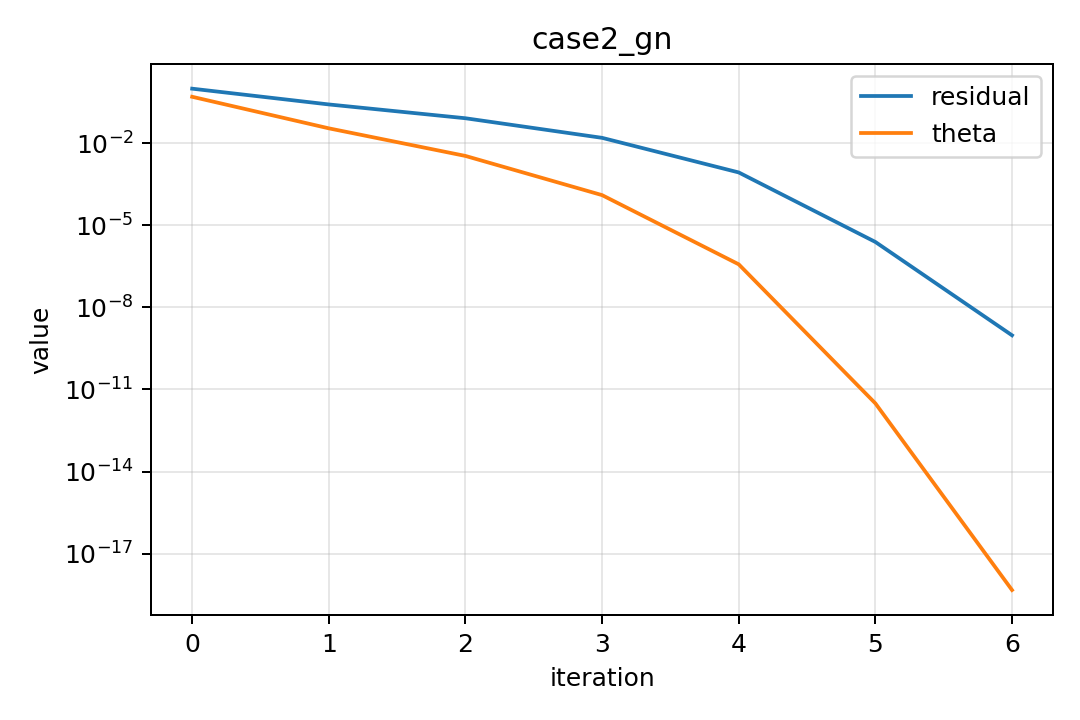
\includegraphics[width=0.72\textwidth]{代码/results/figures/case2_gn_history.png}
\caption{二维终端跟踪算例的残差与目标函数下降曲线}
\label{fig:case2-history}
\end{figure}

\begin{figure}[htbp]
\centering
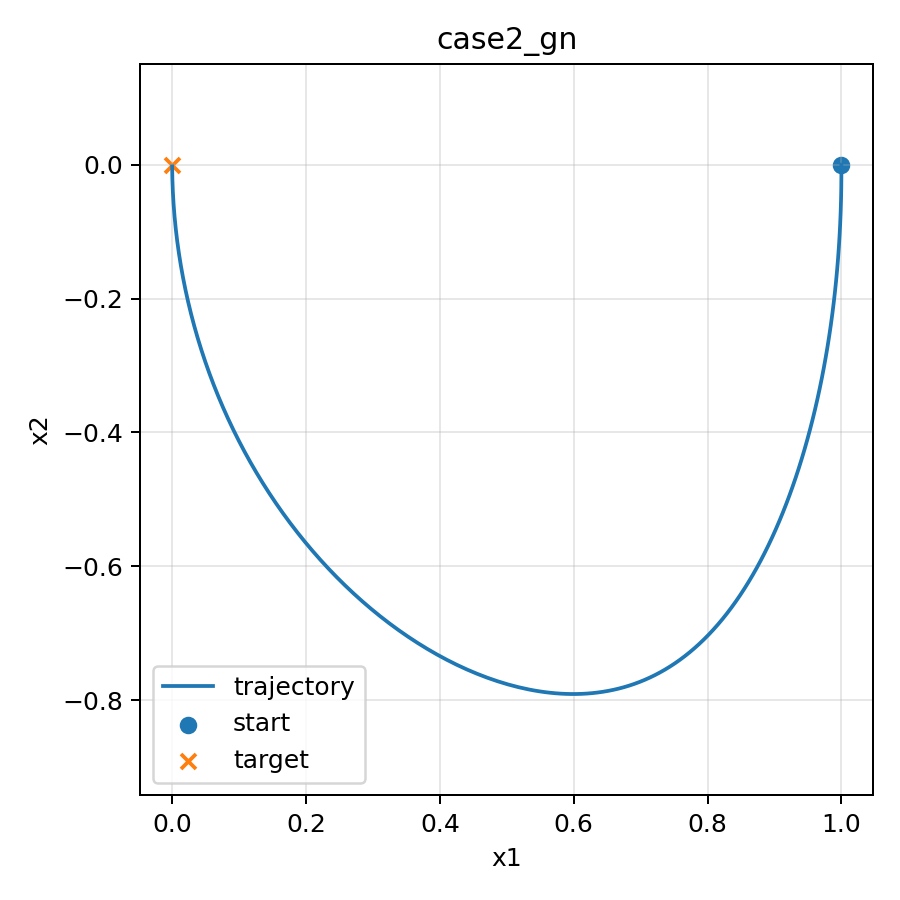
\includegraphics[width=0.62\textwidth]{代码/results/figures/case2_gn_phase.png}
\caption{二维终端跟踪算例的状态相轨线}
\label{fig:case2-phase}
\end{figure}

\begin{figure}[htbp]
\centering
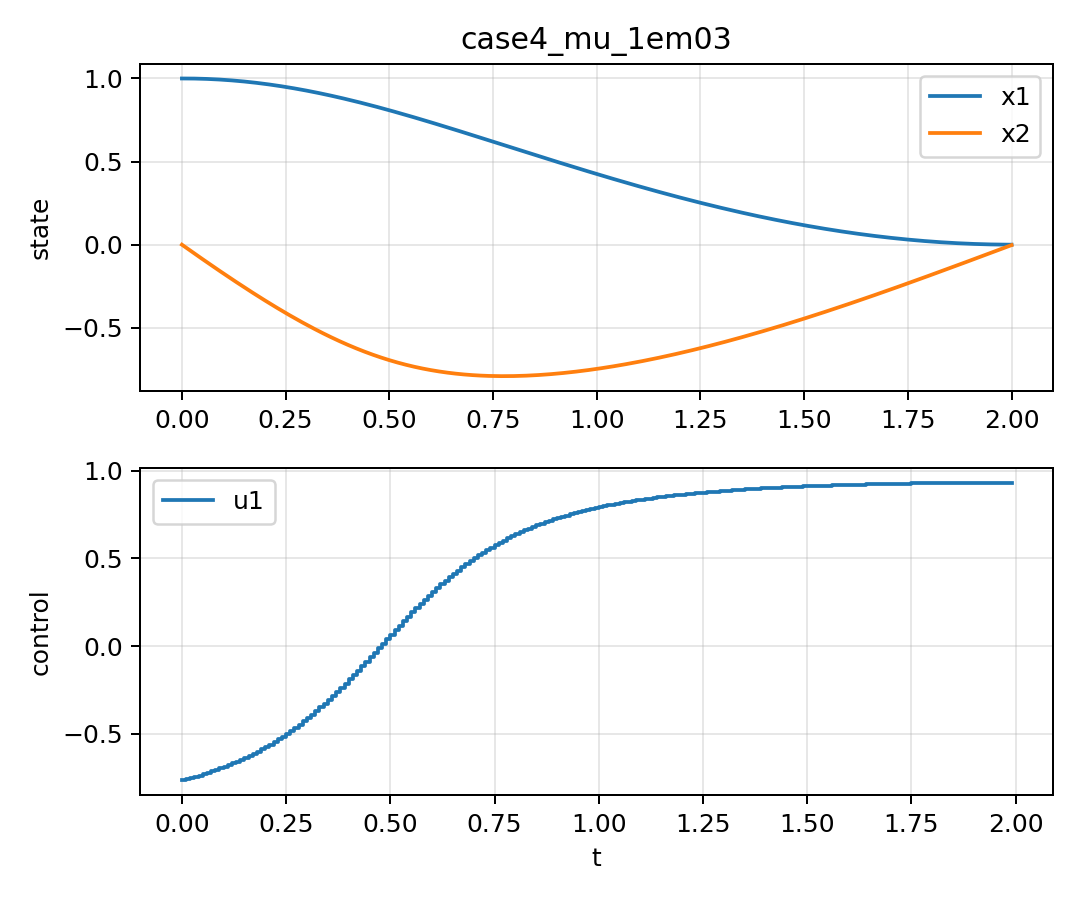
\includegraphics[width=0.72\textwidth]{代码/results/figures/case4_mu_1em03_state_control.png}
\caption{光滑化参数 $\mu=10^{-3}$ 时的状态曲线与控制曲线}
\label{fig:case4-control}
\end{figure}

\subsection{5.9 本章小结}

本章通过多组算例验证了第4章算法的可实现性。二次终端误差算例表明，伴随终端参数 $q$ 可以通过有限维残差最小二乘稳定求解；二维跟踪算例表明，高斯--牛顿方向比梯度方向更适合本文残差方程；仿射终端目标集算例表明，乘子 $\lambda$ 参数化能够有效降低终端约束残差；光滑化对比算例表明，非光滑 bang-bang 控制直接参与有限差分迭代时容易导致不稳定，而适当的光滑化参数能改善收敛行为。实验同时说明，光滑化残差小并不必然意味着原非光滑问题终端误差也小，因此需要同时报告残差和实际终端误差。

\section{第6章 总结与展望}

\subsection{6.1 总结}

本文围绕具有线性动力学的最优控制终端问题的数值解展开研究。首先建立了常系数线性控制系统、允许控制集、可达集、支撑函数以及两个终端型最优控制问题的数学模型；然后在统一的最小化框架下，引入最大化形式伴随变量 $\psi=-p$，将最大值条件表示为支撑函数上的最大化问题；进一步利用线性伴随方程的结构，将未知控制函数转化为有限维伴随终端参数；最后针对二次终端误差问题和带仿射终端目标集约束的线性终端泛函问题，构造了离散递推、残差最小二乘、有限差分 Jacobian、Armijo 线搜索和高斯--牛顿方向组成的数值求解流程。

主要结论如下：

\begin{enumerate}
\item 对线性动力学系统，伴随方程具有线性结构，整条伴随轨线可由终端向量 $q=\psi(T)$ 决定。
\item 通过引入 $\psi=-p$，最小化问题中的控制条件可以统一写成支撑函数的最大化形式。
\item 二次终端误差问题可通过伴随终端条件转化为关于 $q$ 的有限维残差最小二乘问题。
\item 带仿射终端目标集的线性终端泛函问题可通过乘子 $\lambda$ 进行有限维参数化，并以终端约束残差作为数值求解对象。
\item 有限差分 Jacobian、Armijo 线搜索和高斯--牛顿方向构成了可直接实现的参数迭代方法。
\item 对非光滑控制集，可通过光滑化支撑函数改善切换点附近的数值稳定性。
\item 数值实验表明，应同时报告有限维残差和实际终端误差，特别是在光滑化参数较大或直接 bang-bang 迭代时，二者可能呈现不同含义。
\end{enumerate}

\subsection{6.2 展望}

后续研究可以从以下方向展开：

\begin{enumerate}
\item 将线性动力学推广到非线性动力学系统。
\item 考虑含状态约束的终端型最优控制问题。
\item 研究随机扰动或不确定参数下的终端控制问题。
\item 将开环最优控制方法推广到反馈控制或模型预测控制框架。
\item 在高维系统中引入拟牛顿法、共轭梯度法、伴随灵敏度方程或模型降阶方法，提高 Jacobian 计算和迭代求解效率。
\end{enumerate}

\section{参考文献}

\begin{thebibliography}{99}
\bibitem{pontryagin1969}
Л. С. Понтрягин, В. Г. Болтянский, Р. В. Гамкрелидзе, Е. Ф. Мищенко.
\newblock \emph{Математическая теория оптимальных процессов}.
\newblock Москва: Наука, 1969.

\bibitem{kiselev2007}
Ю. Н. Киселёв, С. Н. Аввакумов, М. В. Орлов.
\newblock \emph{Оптимальное управление. Линейная теория и приложения}.
\newblock Москва: Издательский отдел факультета ВМиК МГУ им. М. В. Ломоносова, 2007.

\bibitem{lee1972}
Э. Б. Ли, Л. Маркус.
\newblock \emph{Основы теории оптимального управления}.
\newblock Москва: Наука, 1972.

\bibitem{blagodatskikh2001}
В. И. Благодатских.
\newblock \emph{Введение в оптимальное управление (линейная теория)}.
\newblock Москва: Высшая школа, 2001.

\bibitem{pontryagin1985}
Л. С. Понтрягин.
\newblock Математическая теория оптимальных процессов и дифференциальные игры.
\newblock \emph{Труды Математического института АН СССР}, 1985, т. 169, с. 119--158.

\bibitem{avvakumov1995}
С. Н. Аввакумов, Ю. Н. Киселёв, М. В. Орлов.
\newblock Методы решения задач оптимального управления на основе принципа максимума Понтрягина.
\newblock \emph{Труды Математического института им. В. А. Стеклова}, 1995, т. 211, с. 3--31.

\bibitem{bryson1975}
A. E. Bryson, Y.-C. Ho.
\newblock \emph{Applied Optimal Control: Optimization, Estimation, and Control}.
\newblock Washington: Hemisphere Publishing, 1975.

\bibitem{kirk1970}
D. E. Kirk.
\newblock \emph{Optimal Control Theory: An Introduction}.
\newblock Englewood Cliffs: Prentice-Hall, 1970.

\bibitem{vinter2000}
R. B. Vinter.
\newblock \emph{Optimal Control}.
\newblock Boston: Birkhäuser, 2000.

\bibitem{liberzon2012}
D. Liberzon.
\newblock \emph{Calculus of Variations and Optimal Control Theory: A Concise Introduction}.
\newblock Princeton: Princeton University Press, 2012.

\bibitem{betts2010}
J. T. Betts.
\newblock \emph{Practical Methods for Optimal Control and Estimation Using Nonlinear Programming}.
\newblock Philadelphia: SIAM, 2010.

\bibitem{rao2009}
A. V. Rao.
\newblock A survey of numerical methods for optimal control.
\newblock \emph{Advances in the Astronautical Sciences}, 2009, vol. 135, pp. 497--528.

\bibitem{nocedal2006}
J. Nocedal, S. J. Wright.
\newblock \emph{Numerical Optimization}. 2nd ed.
\newblock New York: Springer, 2006.

\bibitem{kelley1999}
C. T. Kelley.
\newblock \emph{Iterative Methods for Optimization}.
\newblock Philadelphia: SIAM, 1999.
\end{thebibliography}

\end{document}
